\documentclass[11pt]{article}

\usepackage[margin=1in]{geometry}
\usepackage{amsmath, amssymb}
\usepackage{graphicx}
\usepackage{booktabs}
\usepackage{microtype}
\usepackage{hyperref}
\usepackage{xcolor}
\usepackage{tikz}
\usepackage[most]{tcolorbox}
\usetikzlibrary{arrows.meta, positioning, decorations.pathreplacing,
                calc, shapes.geometric, patterns}

\graphicspath{{figures/}}

\hypersetup{colorlinks=true, linkcolor=blue!50!black,
            urlcolor=blue!50!black, citecolor=blue!50!black}

\newtcolorbox{numbersbox}[1][]{
  colback=blue!5, colframe=blue!50!black, fonttitle=\bfseries,
  title=#1, sharp corners, boxrule=0.6pt}

\newtcolorbox{primerbox}[1][]{
  colback=yellow!10, colframe=orange!70!black, fonttitle=\bfseries,
  title=#1, sharp corners, boxrule=0.6pt}

\title{Auditory Superstitious-Perception: results walkthrough}
\author{}
\date{}

\begin{document}
\maketitle
\tableofcontents
\bigskip

%==============================================================================
\section{The experiment}
%==============================================================================

26 college students completed two blocks of $\sim$150 trials each. On every
trial they heard a short noisy audio clip and reported whether it was the
``target'' or the ``distractor''. The underlying target and distractor
clips are essentially noise; chance performance is $0.50$.

The two block types are \texttt{full\_sentence} (the target is replayed at
the start of each trial) and \texttt{imagined\_sentence} (subjects must hold
the target in memory). Subjects were recruited at Oberlin ($n=16$) and
UChicago ($n=10$). Every comparison is reported three ways: each site
alone and pooled (``Unified'').

%==============================================================================
\section{Brief jargon primer}
%==============================================================================

Skip if you already know what a $p$-value, Cohen's $d$, and cosine
similarity are.

\subsection{Accuracy and chance}
Each subject's score is fraction correct, between 0 and 1. If the noise is
truly undiscriminable, scores cluster around $0.50$.

The intuition: imagine flipping a fair coin 150 times and calling each
flip. You will get close to 75 right but almost never exactly 75. By
chance alone you might land at 80/150 ($0.533$) or 70/150 ($0.467$).
That random spread around $0.50$ is what a single subject looks like
under the null. The question for each group is whether the cloud of
subject means sits noticeably to the right of $0.50$ \emph{more often
than that random spread would explain}.

With 150 trials per subject, the standard deviation of an individual
subject's accuracy under the null is roughly $\sqrt{0.25/150} \approx
0.041$. So a single subject scoring $0.54$ is unremarkable; a group of
16 subjects \emph{averaging} $0.526$ is much harder for chance to
produce, because the group mean's standard error shrinks by
$\sqrt{16}$.

\begin{center}
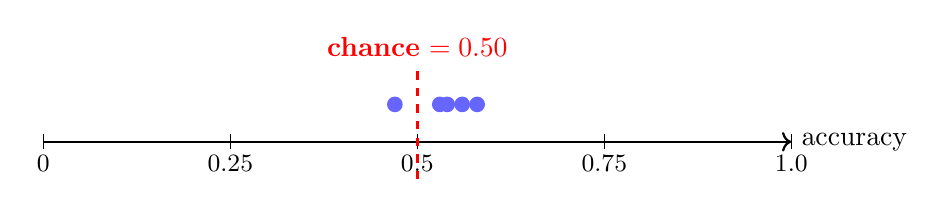
\begin{tikzpicture}[scale=0.95]
  \draw[thick,->] (0,0) -- (10,0) node[right]{accuracy};
  \foreach \x/\lab in {0/0, 2.5/0.25, 5/0.5, 7.5/0.75, 10/1.0}
    \draw (\x,-0.1) -- (\x,0.1) node[below=4pt]{\small \lab};
  \draw[red, very thick, dashed] (5,-0.5) -- (5,1.0)
        node[above, red]{\textbf{chance} $= 0.50$};
  \node[circle, fill=blue!60, inner sep=2pt] at (5.4,0.5) {};
  \node[circle, fill=blue!60, inner sep=2pt] at (5.6,0.5) {};
  \node[circle, fill=blue!60, inner sep=2pt] at (5.8,0.5) {};
  \node[circle, fill=blue!60, inner sep=2pt] at (5.3,0.5) {};
  \node[circle, fill=blue!60, inner sep=2pt] at (4.7,0.5) {};
\end{tikzpicture}
\end{center}

\subsection{The $p$-value}
Probability of a result at least as extreme as the observed one, under
the null hypothesis. Smaller $p$ = more surprising under the null. The
conventional cutoff is $p < 0.05$.

The intuition: pretend the null is true (subjects are guessing). Now
imagine re-running the whole experiment a thousand times in that
imaginary world. The $p$-value is the fraction of those imaginary
replications that would produce a group mean at least as far from
chance as what we actually observed. $p = 0.05$ means \emph{1 in 20
imaginary null-world experiments would look this extreme by accident}.
$p = 0.001$ means $1$ in $1000$.

A $p$-value is \emph{not} the probability that the null is true, and
it is \emph{not} the probability that the effect is real. It is a
statement about how often pure noise would mimic the observation.

When we run many tests (e.g.\ 6 cells in Section~A, 48 correlations in
Section~F) some will land below $0.05$ by accident. Bonferroni
correction divides $\alpha = 0.05$ by the number of tests; so 6 tests
$\Rightarrow$ require $p < 0.0083$, 48 tests $\Rightarrow$ require
$p < 0.001$.

\subsection{Cohen's $d$}
Effect size in units of pooled standard deviation. Rough rule of thumb:
$|d| \approx 0.2$ small, $0.5$ medium, $0.8$ large.

The intuition: $p$-values conflate two things --- how big the effect is,
and how many subjects you ran. Run enough subjects and a tiny effect
will clear $p < 0.05$; run too few and a large effect will miss it.
Cohen's $d$ strips out sample size and tells you the size of the gap
between the observed mean and the null in units of how spread out the
subjects are.

A concrete way to read it: $d = 1.0$ means the observed mean is one
full standard deviation away from the null value. If subjects' scores
formed a bell curve centered on chance, an observed group mean at
$d = 1.0$ would sit out near the edge of that bell, in the region
where only $\sim 16\%$ of single subjects naturally fall. The picture
below shows three null/observed pairs at $d = 0.2, 0.5, 0.8$ ---
notice how much the two distributions still overlap even at $d = 0.8$.

\begin{center}
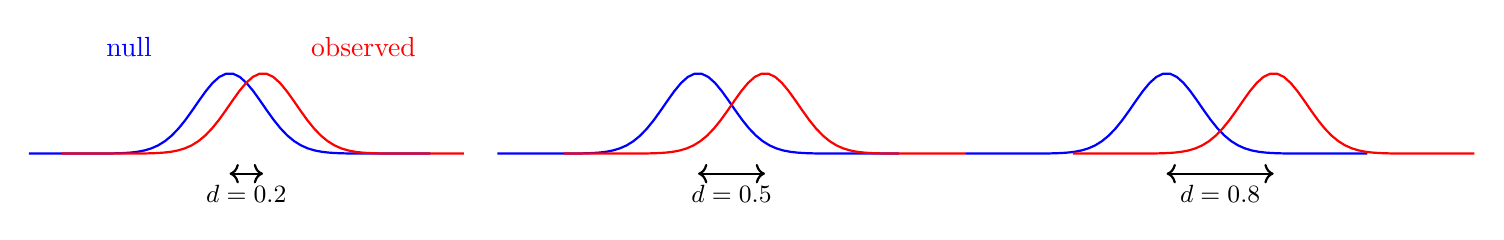
\begin{tikzpicture}[scale=0.85]
  \def\bell#1#2#3{
    \draw[#3, thick] plot[domain=-3:3, samples=60]
      (\x+#1, {1.2*exp(-(\x)^2/0.5)});
  }
  \bell{0}{0}{blue}
  \bell{0.5}{0}{red}
  \node[blue] at (-1.5, 1.6) {null};
  \node[red] at (2, 1.6) {observed};
  \draw[<->, thick] (0, -0.3) -- (0.5, -0.3);
  \node at (0.25, -0.6) {\small $d=0.2$};

  \begin{scope}[xshift=7cm]
    \bell{0}{0}{blue}
    \bell{1}{0}{red}
    \draw[<->, thick] (0, -0.3) -- (1, -0.3);
    \node at (0.5, -0.6) {\small $d=0.5$};
  \end{scope}

  \begin{scope}[xshift=14cm]
    \bell{0}{0}{blue}
    \bell{1.6}{0}{red}
    \draw[<->, thick] (0, -0.3) -- (1.6, -0.3);
    \node at (0.8, -0.6) {\small $d=0.8$};
  \end{scope}
\end{tikzpicture}
\end{center}

\subsection{Cosine similarity}
A waveform or per-subject classification image is a long list of
numbers, i.e.\ a vector. The cosine of the angle between two vectors is
$+1$ if identical direction, $0$ if orthogonal, $-1$ if opposite. We
use it to compare a subject's classification image to the true target
waveform.

The intuition: a subject's \emph{classification image} is built by
averaging the audio waveforms of all the trials they called ``target''
and subtracting the average of trials they called ``distractor''. If
they were guessing, this difference is just averaged noise and points
in a random direction. If they were actually picking up on the target,
this difference should look something like the real target waveform
--- so the angle between their classification image and the true target
should be small, and the cosine close to $+1$.

Why cosine and not raw dot product: cosine ignores how loud or
contrasty the subject's classification image happens to be (its
length) and only asks whether it points in the right direction. Two
subjects with very different overall response biases can both have
$\cos = +0.5$ if their classification images both \emph{shape-match}
the target.

\begin{center}
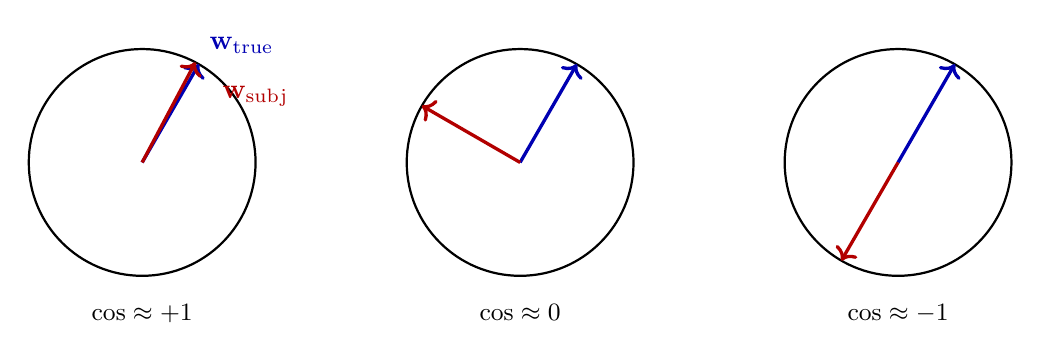
\begin{tikzpicture}[scale=1.2]
  \draw[thick] (0,0) circle (1.2);
  \draw[->, very thick, blue!70!black] (0,0) -- (60:1.2)
        node[above right]{$\mathbf{w}_{\text{true}}$};
  \draw[->, very thick, red!70!black] (0,0) -- (62:1.2);
  \node[red!70!black] at (1.2,0.7) {$\mathbf{w}_{\text{subj}}$};
  \node[below] at (0,-1.4) {\small $\cos \approx +1$};

  \begin{scope}[xshift=4cm]
    \draw[thick] (0,0) circle (1.2);
    \draw[->, very thick, blue!70!black] (0,0) -- (60:1.2);
    \draw[->, very thick, red!70!black] (0,0) -- (150:1.2);
    \node[below] at (0,-1.4) {\small $\cos \approx 0$};
  \end{scope}

  \begin{scope}[xshift=8cm]
    \draw[thick] (0,0) circle (1.2);
    \draw[->, very thick, blue!70!black] (0,0) -- (60:1.2);
    \draw[->, very thick, red!70!black] (0,0) -- (240:1.2);
    \node[below] at (0,-1.4) {\small $\cos \approx -1$};
  \end{scope}
\end{tikzpicture}
\end{center}

\subsection{$d'$ (signal-detection sensitivity)}
$d'$ separates ``can the subject tell target from distractor'' from
``does the subject lean toward saying yes or no''. Two subjects can
both score $0.55$ accuracy, but one might be balanced (hits and
correct rejections both around $0.55$) while the other is biased
(says ``target'' on almost every trial, racking up hits but also
false alarms). $d'$ rewards the first and not the second.

Concretely, $d' = z(\text{hit rate}) - z(\text{false-alarm rate})$.
Null value is $0$. As a sanity check, an accuracy of $0.526$ with no
bias corresponds to $d' \approx 0.13$, matching the Oberlin
full-sentence row in Section~E.\@

\subsection{$\beta_{\text{truetarget}}$ (regression slope on the true target)}
A logistic regression of the subject's per-trial response on the
trial-by-trial dot product between the stimulus waveform and the true
target waveform. A positive slope means \emph{the more the trial's
audio resembled the true target, the more likely the subject was to
call it ``target''}. Null value is $0$. This is a direct test of
target-driven responding, with units of log-odds per unit of
target-similarity.

%==============================================================================
\section{Results}
%==============================================================================

\subsection{Section A: Accuracy vs chance}

\begin{numbersbox}[Section A (\texttt{A\_accuracy\_vs\_chance.csv})]
\centering\small
\begin{tabular}{llrrlrr}
\toprule
block & group & $n$ & mean & 95\% CI & Wilcoxon $p$ & $d$ \\
\midrule
full\_sentence     & UChicago & 10 & 0.504 & $[0.479, 0.530]$ & 0.869  & $+0.09$ \\
full\_sentence     & Oberlin  & 16 & 0.526 & $[0.513, 0.538]$ & 0.0037 & $+0.99$ \\
full\_sentence     & Unified  & 26 & 0.518 & $[0.504, 0.530]$ & 0.019  & $+0.50$ \\
imagined\_sentence & UChicago & 10 & 0.490 & $[0.464, 0.515]$ & 0.611  & $-0.23$ \\
imagined\_sentence & Oberlin  & 16 & 0.510 & $[0.495, 0.526]$ & 0.277  & $+0.31$ \\
imagined\_sentence & Unified  & 26 & 0.502 & $[0.488, 0.517]$ & 0.517  & $+0.06$ \\
\bottomrule
\end{tabular}
\end{numbersbox}

\begin{figure}[h]
\centering
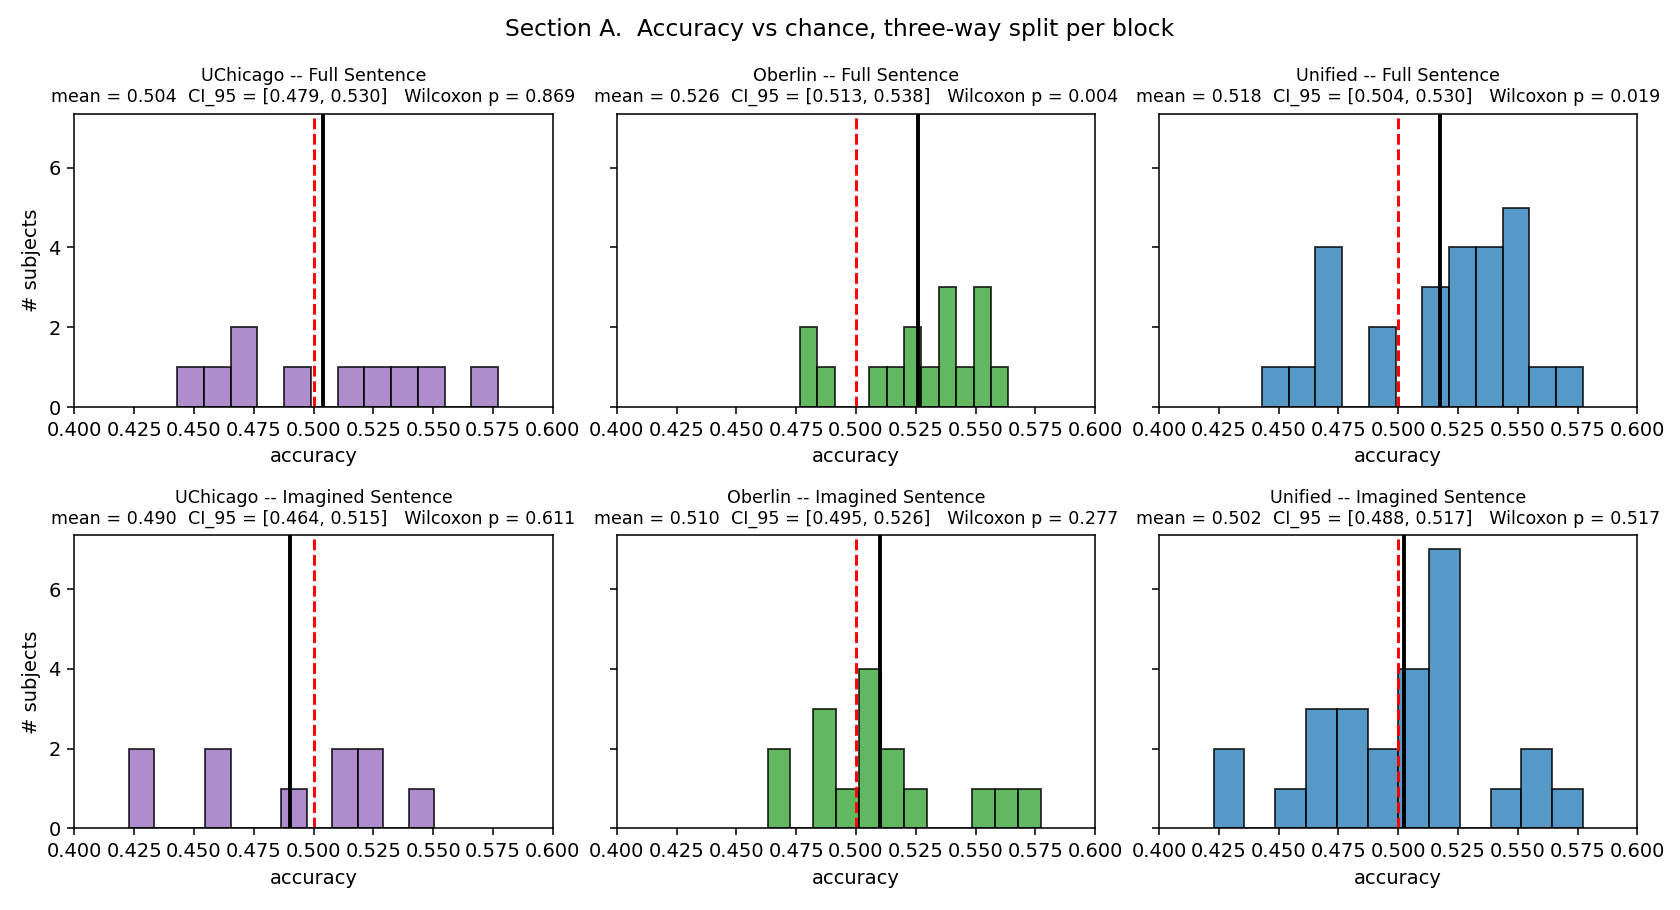
\includegraphics[width=\linewidth]{A_accuracy_vs_chance.png}
\caption{Per-subject accuracy by (block, group). Red dashed = chance
($0.50$); black solid = group mean. Title shows the bootstrap CI on the
mean and the Wilcoxon $p$ vs.\ chance.}
\end{figure}

Bonferroni-corrected threshold across the six tests is
$\alpha = 0.05/6 \approx 0.0083$. Oberlin full-sentence
($p = 0.0037$) clears it; the Unified full-sentence cell
($p = 0.019$) does not.

\subsection{Section B: Full vs Imagined (paired)}

\begin{numbersbox}[Section B (\texttt{B\_full\_vs\_imagined.csv})]
\centering\small
\begin{tabular}{lrrrrrrr}
\toprule
group & $n$ & mean(F) & mean(I) & mean diff & paired Wilcoxon $p$ & perm $p$ & $d$ \\
\midrule
UChicago & 10 & 0.504 & 0.490 & $+0.0141$ & 0.543 & 0.508 & $+0.22$ \\
Oberlin  & 16 & 0.526 & 0.510 & $+0.0159$ & 0.209 & 0.198 & $+0.35$ \\
Unified  & 26 & 0.518 & 0.502 & $+0.0152$ & 0.157 & 0.158 & $+0.29$ \\
\bottomrule
\end{tabular}
\end{numbersbox}

\begin{figure}[h]
\centering
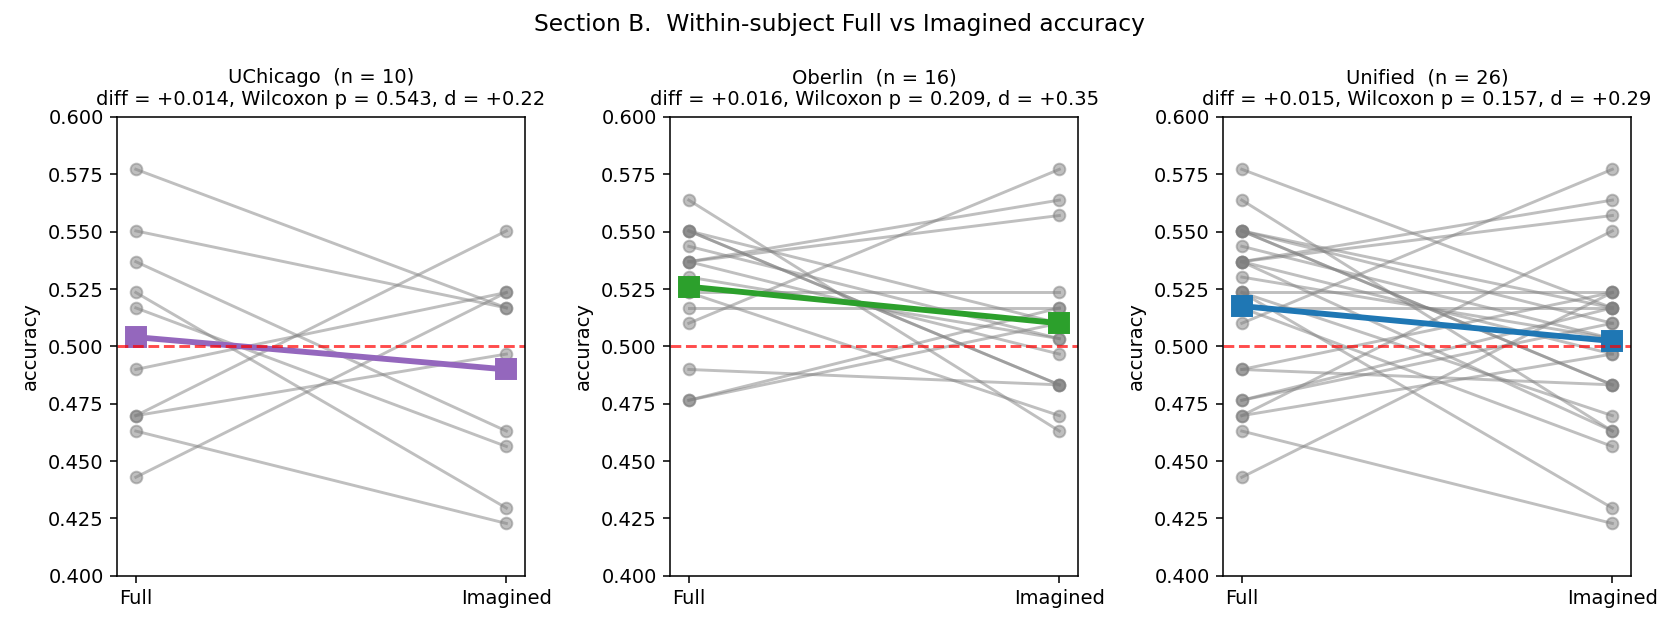
\includegraphics[width=\linewidth]{B_full_vs_imagined.png}
\caption{Per-subject lines connecting Full to Imagined accuracy in each
group; coloured heavy line is the group mean.}
\end{figure}

The mean difference is $+0.0152$ pooled and positive in both sites.
No paired test reaches $p < 0.05$.

\subsection{Section C: Site comparison}

\begin{numbersbox}[Section C (\texttt{C\_site\_comparison.csv})]
\centering\small
\begin{tabular}{lrrrrrrrr}
\toprule
block & $n_O$ & $n_U$ & mean$_O$ & mean$_U$ & diff & MWU $p$ & Welch $p$ & $d$ \\
\midrule
full\_sentence     & 16 & 10 & 0.526 & 0.504 & $+0.0220$ & 0.145 & 0.173 & $+0.65$ \\
imagined\_sentence & 16 & 10 & 0.510 & 0.490 & $+0.0201$ & 0.475 & 0.231 & $+0.54$ \\
\bottomrule
\end{tabular}
\end{numbersbox}

\begin{figure}[h]
\centering
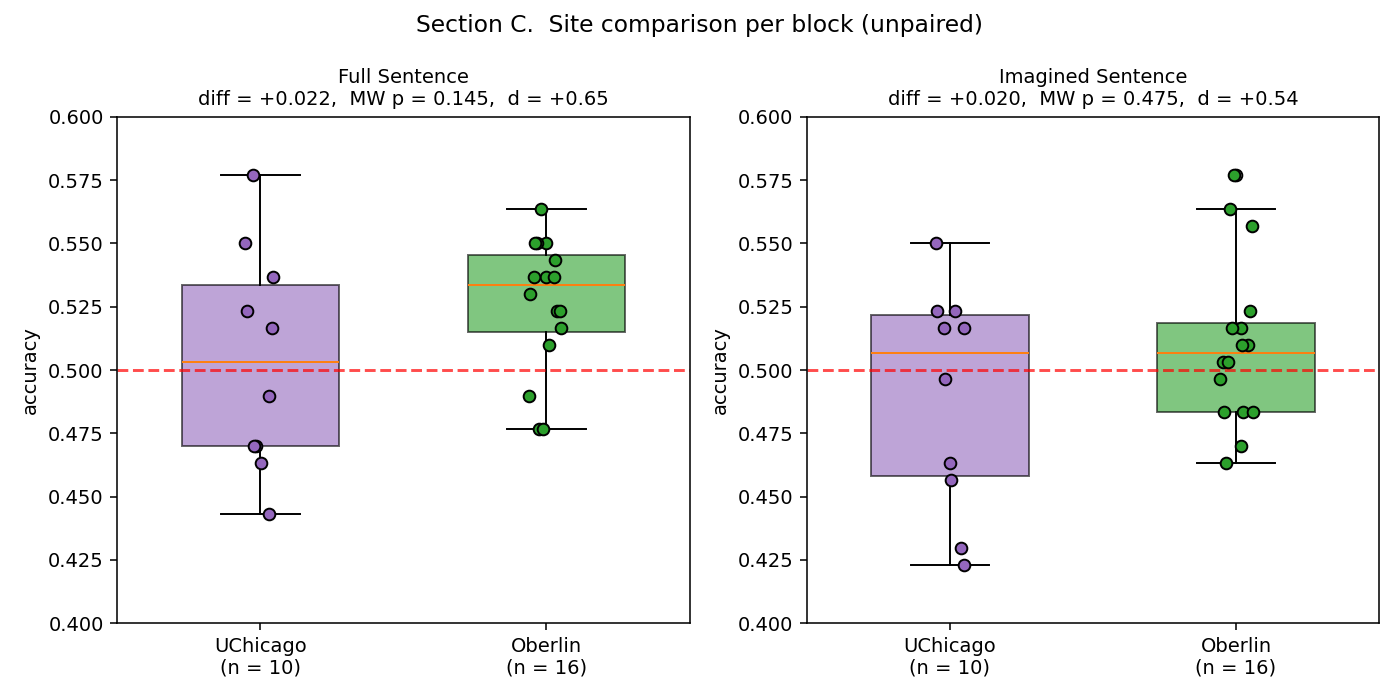
\includegraphics[width=0.85\linewidth]{C_site_comparison.png}
\caption{Per-block boxplots, Oberlin vs.\ UChicago, with overlaid
jittered subject points.}
\end{figure}

Oberlin is numerically higher than UChicago in both blocks by
$\approx 0.02$. Neither between-site comparison reaches $p < 0.05$.

\subsection{Section D: Block order}

\begin{numbersbox}[Section D selected rows (\texttt{D\_block\_order.csv})]
\centering\small
\begin{tabular}{llrrrrrr}
\toprule
block & group & $n_{B1}$ & $n_{B2}$ & mean(B1) & mean(B2) & MWU $p$ & $d$ \\
\midrule
full\_sentence     & Oberlin  &  5 & 11 & 0.519 & 0.529 & 0.493 & $+0.35$ \\
imagined\_sentence & Oberlin  & 11 &  5 & 0.500 & 0.532 & 0.078 & $+1.03$ \\
\bottomrule
\end{tabular}
\end{numbersbox}

In the Oberlin imagined block, subjects who completed it second
($n_{B2}=5$) averaged $0.532$, vs $0.500$ for those who completed it
first ($n_{B1}=11$); MWU $p = 0.078$, $d = +1.03$. All other
block-order cells have $p > 0.4$.

\subsection{Section E: Convergent metrics, full-sentence block}

\begin{numbersbox}[Section E (\texttt{E\_convergent\_full\_sentence.csv})]
\centering\small
\begin{tabular}{llrrrr}
\toprule
group & metric & mean & 95\% CI & Wilcoxon $p$ & $d$ \\
\midrule
Oberlin  & d$'$              & $+0.137$ & $[+0.069, +0.200]$ & 0.0013 & $+0.99$ \\
Oberlin  & accuracy          & $+0.526$ & $[+0.513, +0.538]$ & 0.0037 & $+0.99$ \\
Oberlin  & cos(CI, true)     & $+0.056$ & $[+0.029, +0.083]$ & 0.0013 & $+1.00$ \\
Oberlin  & beta\_truetarget  & $+0.232$ & $[+0.118, +0.340]$ & 0.0027 & $+0.99$ \\
\midrule
UChicago & d$'$              & $+0.021$ & $[-0.106, +0.153]$ & 0.846  & $+0.09$ \\
UChicago & cos(CI, true)     & $-0.002$ & $[-0.059, +0.056]$ & 1.000  & $-0.02$ \\
UChicago & beta\_truetarget  & $+0.042$ & $[-0.159, +0.248]$ & 0.846  & $+0.12$ \\
\midrule
Unified  & d$'$              & $+0.093$ & $[+0.023, +0.159]$ & 0.013  & $+0.51$ \\
Unified  & cos(CI, true)     & $+0.034$ & $[+0.004, +0.063]$ & 0.025  & $+0.43$ \\
Unified  & beta\_truetarget  & $+0.159$ & $[+0.047, +0.267]$ & 0.016  & $+0.55$ \\
\bottomrule
\end{tabular}
\end{numbersbox}

\begin{figure}[h]
\centering
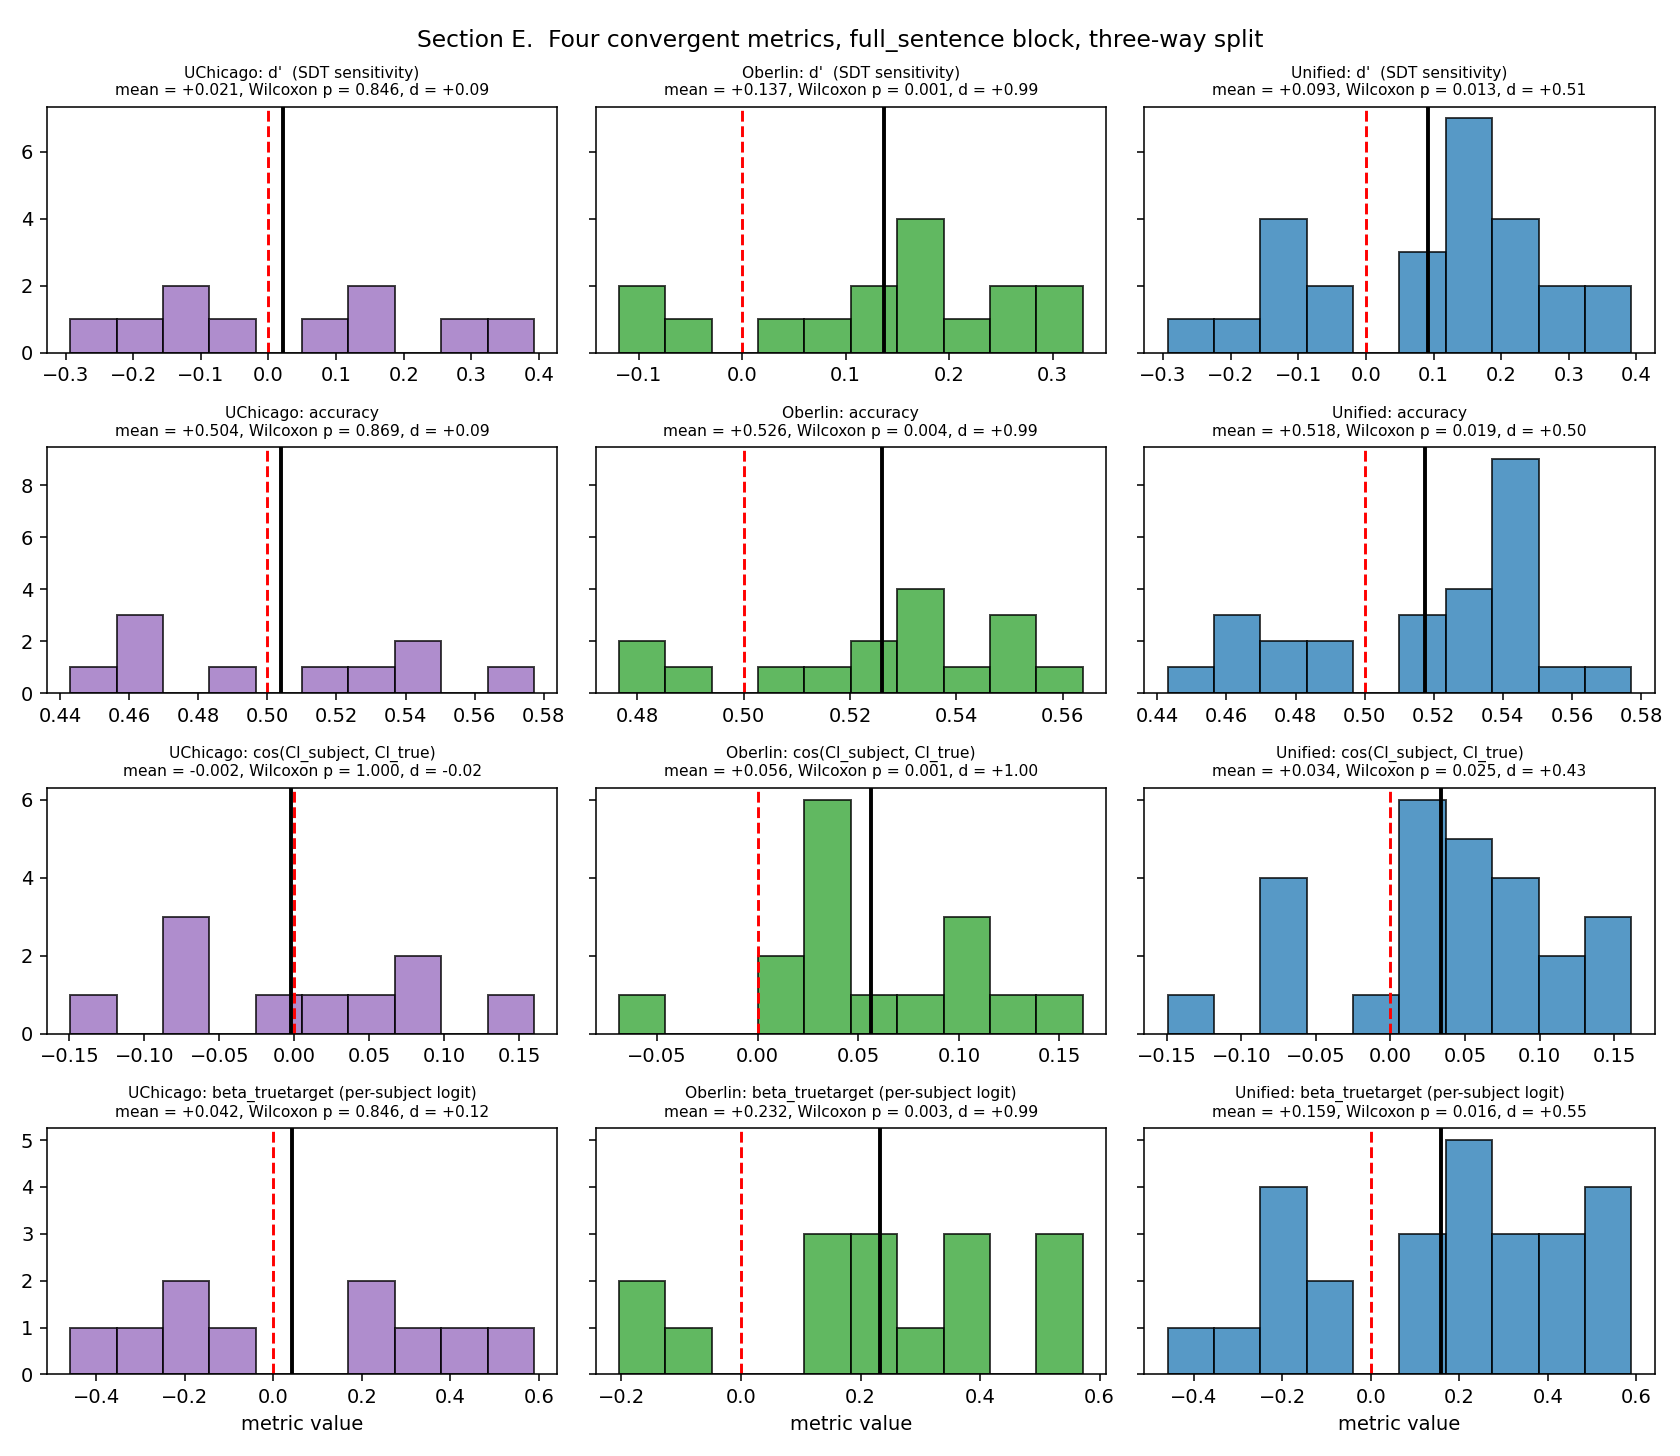
\includegraphics[width=\linewidth]{E_convergent_full_sentence.png}
\caption{Each row is a metric, each column a group. Red dashed = null
value (0 or 0.5); black solid = observed mean.}
\end{figure}

At Oberlin all four metrics yield $p \le 0.0037$ and $d \approx 1.0$.
At UChicago all four are non-significant with $|d| \le 0.12$. Pooled,
all four yield $p \in [0.013, 0.025]$ and $d \in [0.43, 0.55]$.

\subsection{Section F: Questionnaire correlations}

48 Spearman correlations (8 questionnaires $\times$ 2 blocks $\times$
3 groups). Bonferroni threshold $p < 0.001$. None survive correction.
Tables: \texttt{F\_questionnaire\_spearman.csv}; figures:
\texttt{F\_quest\_vs\_accuracy\_full\_sentence.png},
\texttt{F\_quest\_vs\_accuracy\_imagined\_sentence.png}.

%==============================================================================
\section{Further analyses available with the existing data}
%==============================================================================

\subsection{Trial-by-trial mixed-effects modelling}

The current per-subject summaries collapse $\sim$150 trials per block
into a single mean. A mixed-effects logistic regression on raw trials,
with subject as a random effect, would use the within-subject trial
variance directly.

\subsection{Bayesian re-analysis of trending comparisons}

For comparisons with $0.05 < p < 0.20$ (Section~B Full--Imagined paired,
Section~C site differences), Bayes factors quantify the evidence ratio
between $H_1$ and $H_0$ rather than only rejecting $H_0$.

\subsection{Within-subject correlations between convergent metrics}

The four Section~E metrics are tested independently. Computing the
per-subject correlation matrix between $d'$, accuracy, $\cos(\mathrm{CI},
\text{true})$, and $\beta_{\text{truetarget}}$ tests whether they are
driven by a single latent perceptual ability.

\subsection{Spectral classification image}

A 32-band spectral analogue of the time-domain classification image: for
each subject, fit per-band weights and compute the cosine with the true
target's per-band spectrum.

\begin{center}
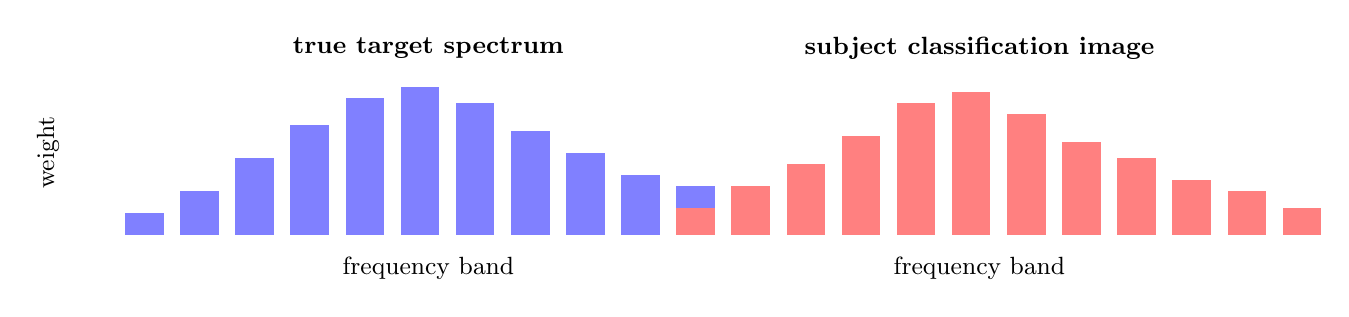
\begin{tikzpicture}[scale=0.7]
  \foreach \x/\h in {1/0.4, 2/0.8, 3/1.4, 4/2.0, 5/2.5, 6/2.7,
                     7/2.4, 8/1.9, 9/1.5, 10/1.1, 11/0.9, 12/0.6}
    \fill[blue!50] (\x,0) rectangle (\x+0.7, \h);
  \node at (6.5,-0.6) {\small frequency band};
  \node[rotate=90] at (-0.4,1.5) {\small weight};
  \node at (6.5,3.4) {\small \textbf{true target spectrum}};

  \begin{scope}[xshift=10cm]
    \foreach \x/\h in {1/0.5, 2/0.9, 3/1.3, 4/1.8, 5/2.4, 6/2.6,
                       7/2.2, 8/1.7, 9/1.4, 10/1.0, 11/0.8, 12/0.5}
      \fill[red!50] (\x,0) rectangle (\x+0.7, \h);
    \node at (6.5,-0.6) {\small frequency band};
    \node at (6.5,3.4) {\small \textbf{subject classification image}};
  \end{scope}
\end{tikzpicture}
\end{center}

\subsection{Block-order follow-up in the Oberlin imagined block}

Trial-resolved analysis of the $n_{B2}=5$ vs $n_{B1}=11$ split: e.g.\
within-block accuracy time course, and whether the $+0.032$ mean
difference is concentrated in early or late trials of the block.

\subsection{Stimulus-level analyses}

Per-stimulus accuracy across the audio set, to test whether particular
target/distractor pairs drive the Oberlin full-sentence effect.
Building blocks for this exist in \texttt{stimuli-analyses/}
(classification-image, spectral logistic, etc.).

\end{document}
